\documentclass[conference]{IEEEtran}
\IEEEoverridecommandlockouts
% The preceding line is only needed to identify funding in the first footnote. If that is unneeded, please comment it out.
%Template version as of 6/27/2024

\usepackage{cite}
\usepackage{amsmath,amssymb,amsfonts}
\usepackage{algorithmic}
\usepackage{graphicx}
\usepackage{textcomp}
\usepackage{xcolor}
\def\BibTeX{{\rm B\kern-.05em{\sc i\kern-.025em b}\kern-.08em
    T\kern-.1667em\lower.7ex\hbox{E}\kern-.125emX}}
\begin{document}

\title{Generalized Kinodynamic Motion Planning for Autonomous Battlebots}

\author{\IEEEauthorblockN{Omri Zvi Green}
\IEEEauthorblockA{\textit{Robotics Engineering} \\
\textit{Worcester Polytechnic Institute}\\
Worcester, Massachusetts, United States of America \\
ozgreen@wpi.edu}}

\maketitle

\begin{abstract}
This paper presents a novel kinodynamic planning framework for autonomous combat robots ("battlebots") that generalizes across different drive systems and weapon configurations. We address the unique challenges of autonomous battle robot navigation, including adversarial environments, weapon-specific constraints, and real-time planning requirements. Our approach models battlebots as differential drive systems with varying weapon dynamics, enabling unified motion planning regardless of specific robot configuration. We develop a comprehensive kinodynamic model that accounts for both locomotion and weapon forces, then benchmark five different planning algorithms (PRM, RG-RRT, ST-RRT*, RRT, and KPIECE1) across six robot configurations in simulated combat scenarios. Results demonstrate that our generalized approach enables effective real-time motion planning for autonomous battlebots while satisfying the specific kinodynamic constraints of each robot type. This work contributes to the emerging field of autonomous combat robotics by providing a foundational planning framework that can be applied to a wide variety of battle robot designs without requiring robot-specific algorithm development.
\end{abstract}

\begin{IEEEkeywords}
Combat Robotics, BattleBot, Beetle Weight, Kinodynamic Planning
\end{IEEEkeywords}

\section{Introduction}
The sport of combat robotics or Battle Bots is a relatively new phenomenon, with the first competition taking place in 1989, the MileHiCon CritterCrunch \cite{b1}.  The essence of the sport is similar a mix of the gladiator fights of Rome and modern MMA, at one of the most popular events, the National Havoc Robotics League, the robots continue fighting until one of the following scenarios take place:
\begin{enumerate}
\item{The time limit is reached \cite{b2}}
\item{One of the robots is completely disabled or "Knocked Out" \cite{b2}}
\item{An operator of one of the robot concedes the match or "Taps Out" \cite{b2}}
\item{There is a Arena Failure, meaning the arena was broken by one of the robots \cite{b2}}
\item{Both robots are entangled and unable to be separated \cite{b2}}
\end{enumerate} 
In scenarios where the winner is unclear such as in scenarios 1, 4, or 5, the winner is decided by a Judges decision where they evaluate who the winner is based on the 3 following criteria:
\begin{enumerate}
\item{Robot Functionality: How well each robot works at the end of the fight \cite{b2}}
\item{Aggression: How much each robot is attacking the opponent \cite{b2}}
\item{Control: How much each robot "controls" the fight, such as pinning them against the wall \cite{b2}}
\end{enumerate}
With these criteria in place we can determine that the optimal general planner for automating a combat robot,, we must primarily focus on one strategy, attacking the opponent as much as possible overwhelming them with constant attacks.  After all the best defense is a good offense.

\section{Related Works}

To create an generalized kinodynamic planner capable of controlling a wide variety of different Battle Bots at competitions such as the National Havoc Robotics League (NHRL) or BattleBots we must not only understand the taxonomy of combat robots, understanding how they move, and how they fight; we must also understand how existing kinodynamic models of robots with similar drive systems, as well as examine existing examples of autonomous battle bots.

\subsection{A Taxonomy Of Combat Robots}
\subsubsection{Drive Systems}

A combat robot's drive system can usually be described as being driven by a form differential drive, they are typically powered by 2 separate drive motors due to the limited weight allowed for each robot, one example of a differential robot is Very Original, a four wheel drive (4WD) robot, which is shown going in a circle below:
\begin{figure}[htp]
\centering
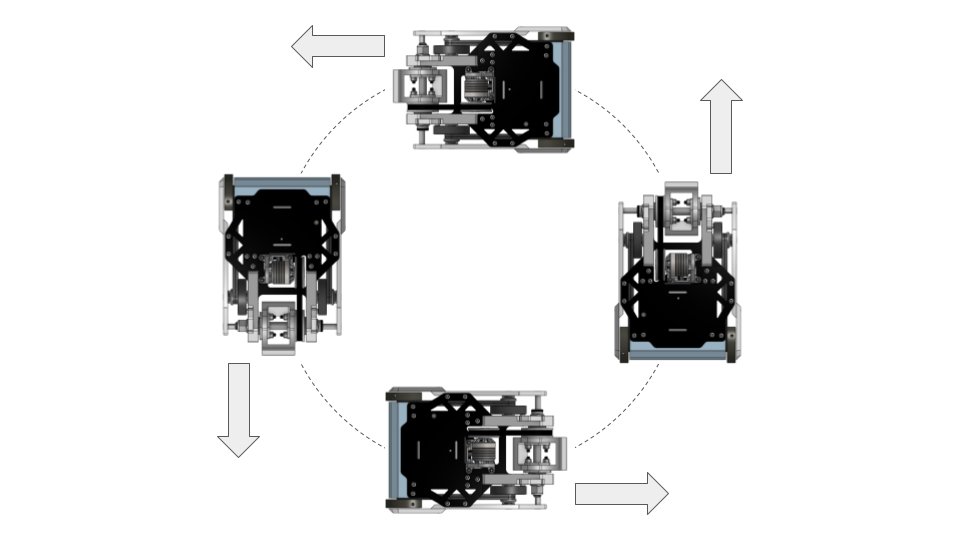
\includegraphics[scale=0.3]{Differential Drive 4WD.png}
\caption{Very Original following a circular path}
\label{Very Original Following a circular path}
\end{figure} 

Other examples of differential drive based methods include two wheel drive robots (2WD), shuffler driven robots, and Jansen Linkage based drive systems.  These methods are shown in the respective robots shown below, Double Stuffed, Blunder, and Pawsitively Hissterical.
\begin{figure}[htp]
\centering
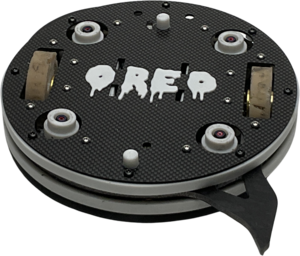
\includegraphics[scale=0.4]{doublestuffed.png}
\caption{Double Stuffed: 2 Wheel Drive \cite{b2}}
\label{Double Stuffed: 2 Wheel Drive}
\end{figure}

\begin{figure}[htp]
\centering
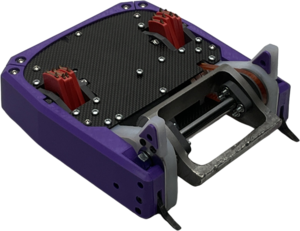
\includegraphics[scale=0.4]{blunder.png}
\caption{Blunder: Shuffler Drive}
\label{Blunder: Shuffler Drive}
\end{figure}

\begin{figure}[htp]
\centering
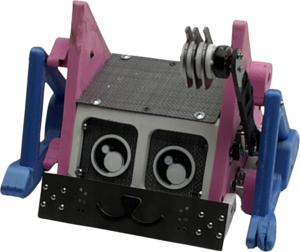
\includegraphics[scale=0.4]{pawsitivelyhissterical.png}
\caption{Pawsitively Hissterical: Jansen Linkage Drive \cite{b2}}
\label{Pawsitively Hissterical: Jansen Linkage Drive}
\end{figure}

There are also other kinds of drive systems used in combat robotics, but they tend to be far less common, examples include true walkers such as Clockwork Princess which are legged robots, Melty Brains such as Project Liftoff which typically spin incredibly quickly and by using an onboard processor and a inertial measurement unit they can be controlled as if they were a point robot, and Swerve Drive robots such as Shifty which work by rotating their wheels along the Z-axis to allow better control at the cost of additional weight.  Each of these robots is shown below:

\begin{figure}[htp]
\centering
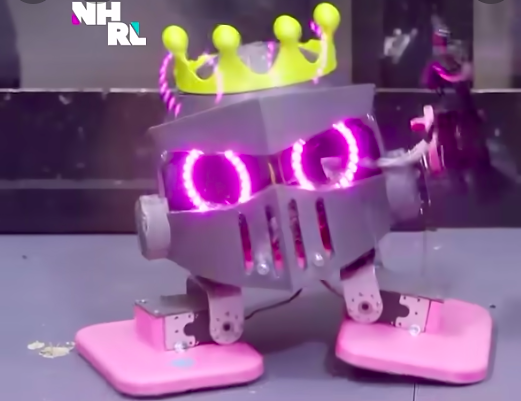
\includegraphics[scale=0.3]{clockworkprincess.png}
\caption{Clockwork Princess: True Walker \cite{b4}}
\label{Clockwork Princess: True Walker}
\end{figure}

\begin{figure}[htp]
\centering
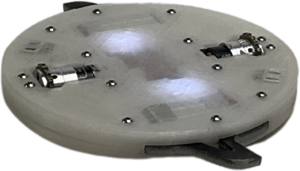
\includegraphics[scale=0.4]{projectliftoff.png}
\caption{Project Liftoff: Melty Brain \cite{b2}}
\label{Project Liftoff: Melty Brain}
\end{figure}

\begin{figure}[htp]
\centering
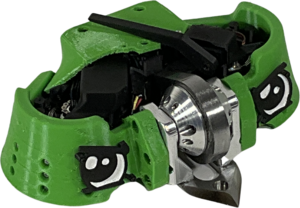
\includegraphics[scale=0.4]{shifty.png}
\caption{Shifty: Swerve Drive \cite{b2}}
\label{Shifty: Swerve Drive}
\end{figure}

\subsubsection{Weapon Types}

While a battle bot must be able to move, they must also be able to fight, meaning that over the years people have developed a wide variety of weapon types.  Due to this will be fitting these weapons into 3 separate categories based on shared features which will be gone over in separate paragraphs.
\begin{enumerate}
\item{Vertical Spinners}
\item{Horizontal Spinners}
\item{Non-Spinning Weapons}
\end{enumerate}

Vertical Spinners are a weapon type that can be described mathematically as a cylinder rotating with its axis of rotation being in the x or y axis in a 3 dimensional space.  Vertical Spinners can then be split into two more categories, which we will call direct, and non-direct.  A direct vertical spinner operates by hitting an opposing robot with a spinning weapon when it initially contacts the opponent, examples of these kinds of weapons are beater bars, drum spinners, drisks, and traditional vertical spinners.  These are mounted on the robots, Eruption, Necromancer, Red Panda, and Blink which are shown below:

\begin{figure}[htp]
\centering
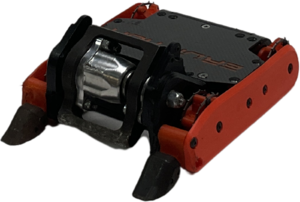
\includegraphics[scale=0.4]{eruption.png}
\caption{Eruption: Beater Bar \cite{b2}}
\label{Eruption: Beater Bar}
\end{figure}

\begin{figure}[htp]
\centering
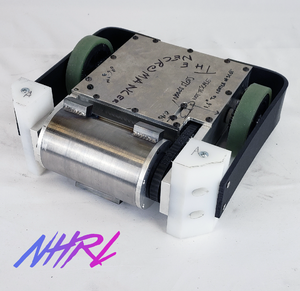
\includegraphics[scale=0.4]{necromancer.png}
\caption{Necromancer: Drum Spinner \cite{b2}}
\label{Necromancer: Drum Spinner}
\end{figure}

\begin{figure}[htp]
\centering
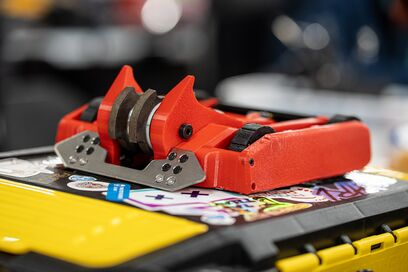
\includegraphics[scale=0.4]{redpanda.jpg}
\caption{Red Panda: Drisk \cite{b2}}
\label{Red Panda: Drisk}
\end{figure}

\begin{figure}[htp]
\centering
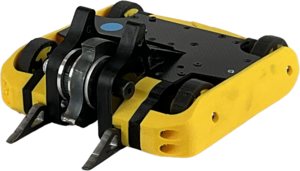
\includegraphics[scale=0.4]{blink.png}
\caption{Blink: Traditional Vertical Spinner \cite{b2}}
\label{Blink: Traditional Vertical Spinner}
\end{figure}

A Non-direct vertical spinner is a vertical spinner that spins up to speed and then is actuated in some way to hit a robot in more venerable areas, typically the top or bottom of the robot.  Examples of this kind of weapon include robots like Chippy use a hammersaw which works by spinning up the vertical spinner to a high speed then hit the top of the opponent as hard as they can to reach vulnerable electronics, saw bots such as Mako work similarly to hammersaws, except they are actuated by a servo allowing them saw through the top of the robot, and lastly a brand new type of weapon used on the robot Juxtaposition, which we will call a inverse hammersaw due to the fact it operates similarly to a hammersaw where it aims to hit the bottom of a robot rather than the top.

\begin{figure}[htp]
\centering
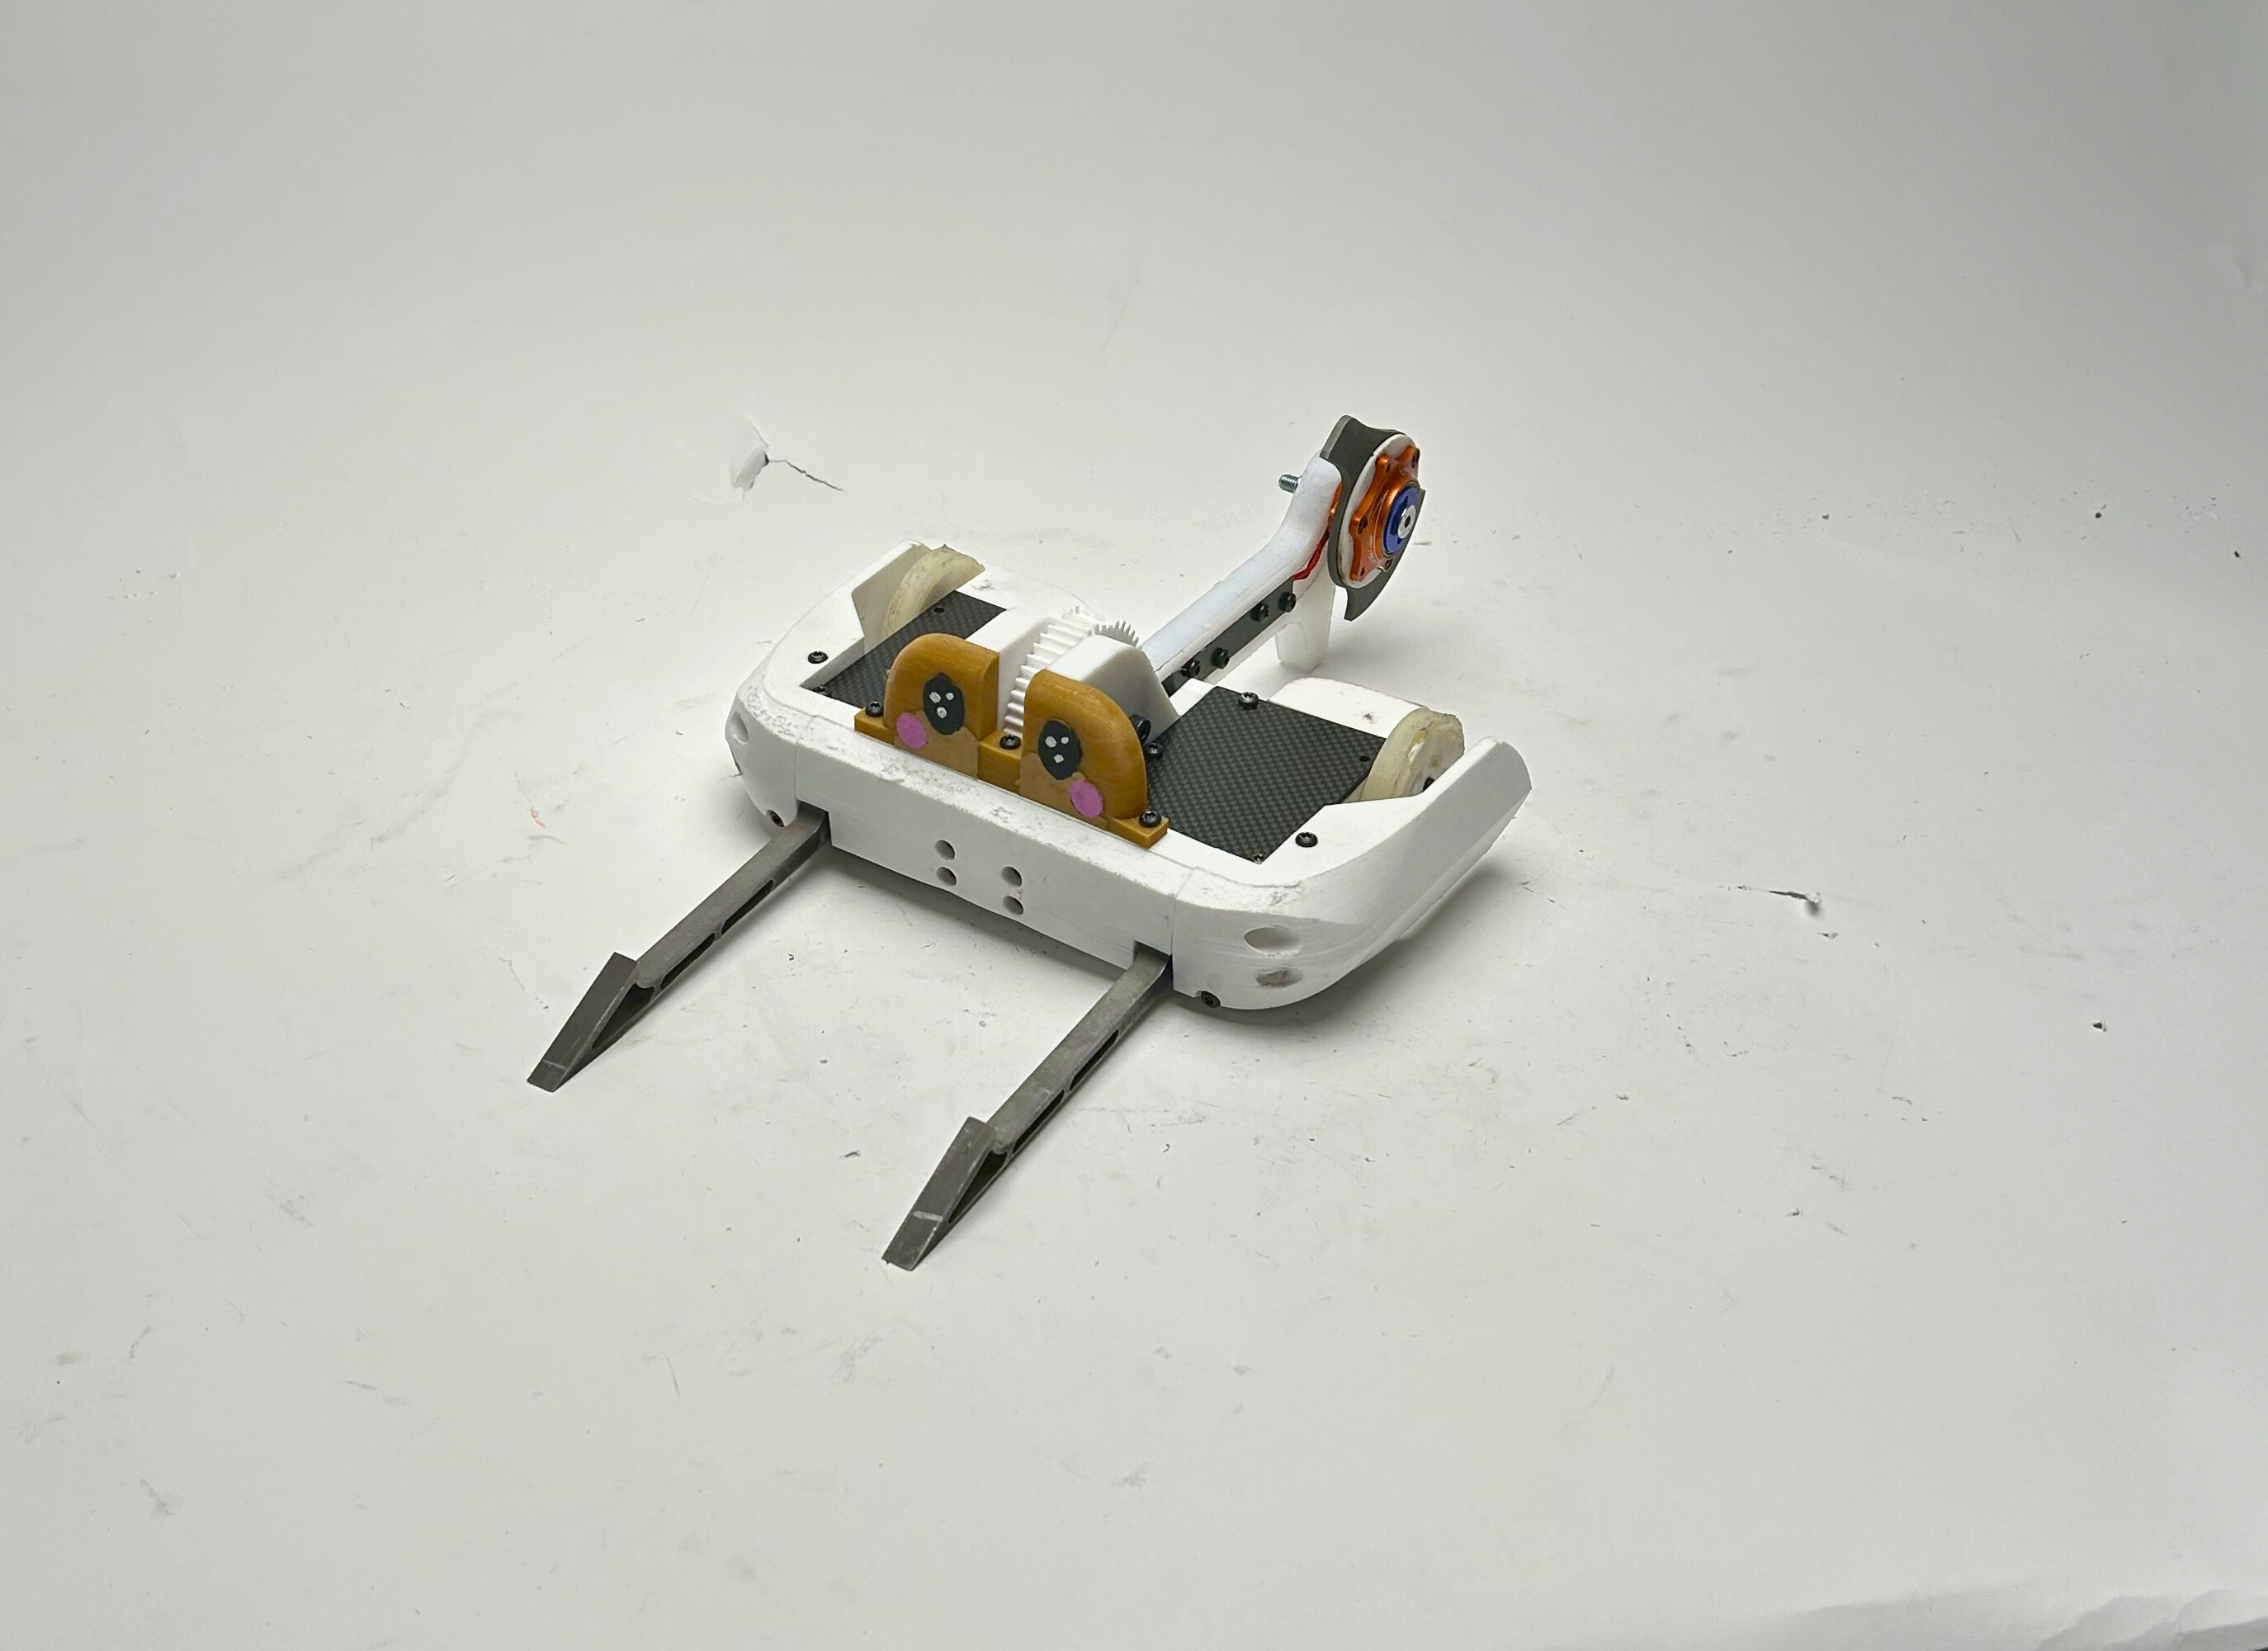
\includegraphics[scale=0.05]{chippy.jpg}
\caption{Chippy: Hammersaw \cite{b2}}
\label{Chippy: Hammersaw}
\end{figure}

\begin{figure}[htp]
\centering
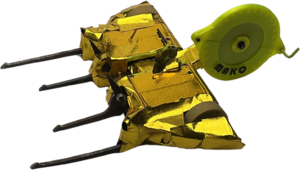
\includegraphics[scale=0.4]{mako.png}
\caption{Mako: Saw \cite{b2}}
\label{Mako: Saw}
\end{figure}

\begin{figure}[htp]
\centering
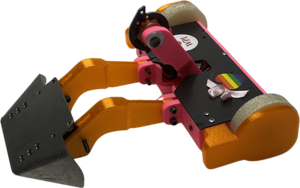
\includegraphics[scale=0.4]{juxtaposition.png}
\caption{Juxtaposition: Inverse Hammersaw \cite{b2}}
\label{Juxtaposition: Inverse Hammersaw}
\end{figure}

\newpage

Horizontal Spinners can be mathematically described similarly to a vertical spinner except that the axis of rotation of the weapon is in the Z-axis in a 3d environment rather than perpendicular to it.  Examples of this kind of spinner are typically categorized by where they lie in relation to the top and bottom of the robot, examples of these include undercutters such as Explosion has its weapon lie under the main body of the robotmidcutters such as The Throngler has its weapon lie in the middle of the robot, and overcutters such as Budget Extinction has their weapon lie above the main body of the robot.  There are also ring spinners such as Double Stuffed which use a ring rotating around the center as their weapon, there are also shell-spinners such as Chonkiv which spin their armor to function as their weapon.

\begin{figure}[htp]
\centering
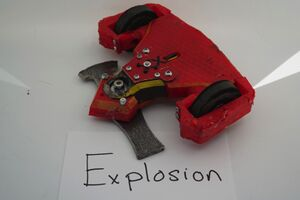
\includegraphics[scale=0.4]{explosion.jpg}
\caption{Explosion: Undercutter \cite{b2}}
\label{Explosion: Undercutter}
\end{figure}

\begin{figure}[htp]
\centering
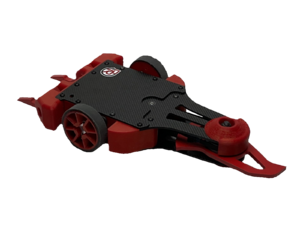
\includegraphics[scale=0.4]{throngler.png}
\caption{The Throngler: Midcutter}
\label{The Throngler: Midcutter}
\end{figure}

\begin{figure}[htp]
\centering
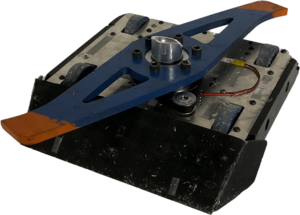
\includegraphics[scale=0.4]{budgetextinction.png}
\caption{Budget Extinction: Overcutter \cite{b2}}
\label{Budget Extinction: Overcutter}
\end{figure}

\begin{figure}[htp]
\centering
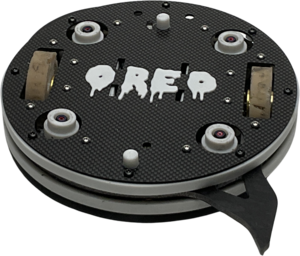
\includegraphics[scale=0.4]{doublestuffed.png}
\caption{Double Stuffed: Ring Spinner \cite{b2}}
\label{Double Stuffed: Ring Spinner}
\end{figure}

\begin{figure}[htp]
\centering
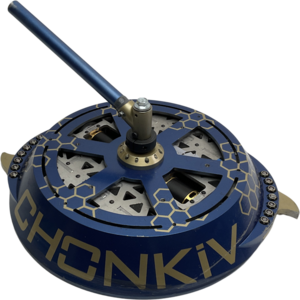
\includegraphics[scale=0.4]{chonkiv.png}
\caption{Chonkiv: Shell Spinner \cite{b2}}
\label{Chonkiv: Shell Spinner}
\end{figure}
\newpage

While spinning weapons are the most common type of weapon on a combat robot, there are a few kinds of non-spinning weapon.  These do not impart damage through hitting a robot with a rotating weapon, rather they do something else to either cause damage or ensure control.  Examples of non-spinning weapons include flamethrowers such as the one used on Clyde, flippers such as Bison work by launching the opponent into the air with an actuated plate, while lifters such as Master Control Bot simply lift their opponents up so they are temporarily ineffective.

\begin{figure}[htp]
\centering
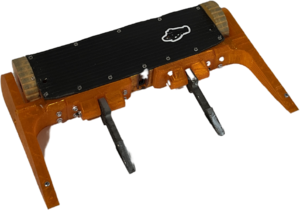
\includegraphics[scale=0.4]{clyde.png}
\caption{Clyde: Flamethrower \cite{b2}}
\label{Clyde: Flamethrower}
\end{figure}

\begin{figure}[htp]
\centering
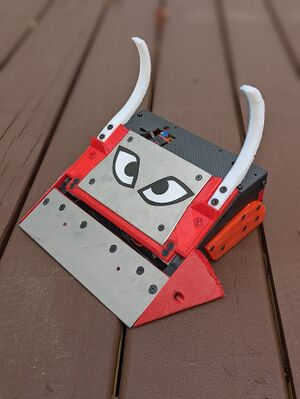
\includegraphics[scale=0.4]{bison.jpg}
\caption{Bison: Flipper \cite{b2}}
\label{Bison: Flipper}
\end{figure}

\begin{figure}[htp]
\centering
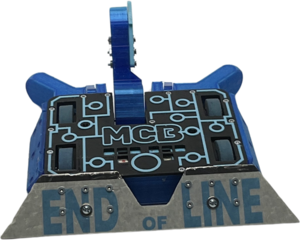
\includegraphics[scale=0.4]{mcbmastercontrolbot.png}
\caption{Master Control Bot: Lifter \cite{b2}}
\label{Master Control Bot: Lifter}
\end{figure}

\newpage

\subsection{Kinodynamic Planner}
According to the paper "Kinodynamic Motion Planning" which first created a practical Kinodynamic Motion Planning algorithm in 1993 \cite{b3}, "The kinodynamic planning problem is to synthesize a robot motion subject to simultaneous kinematic constraints, such as avoiding obstacles, and dynamics constraints, such as modulus bounds on velocity, acceleration, and force."\cite{b3}, essentially it is the problem on how to calculate the most efficient path to a goal while taking into account how the robot moves and is affected by forces imparted on it by said movements.  This is in contrast to other forms of motion planning which ignore the limitations on the robot, this can potentially lead to situations where the motion plan cannot be completed by the robot because it is unable to complete the path.  

\subsection{Existing Autonomous Battle Bots}

In the context of autonomous battle bots the fact that most planners do not take take robot kinodynamics directly affects their design necessitating either specific robot architectures or the use of flywheels.  While this is not an issue in the case of autonomous Melty Brains such as Deep Melt, the first fully autonomous battle bot to compete at the National Havoc Robotics League, however, it doesn't do any planning in an interview with its creator he said that "... if an opponent like brings an IR flashlight and shines it at us, you gave us a beacon to you"\cite{b5} implying that the robot simply seeks out the area where the IR reflects the most from its IR mapping system.  Especially considering the fact that as a Melty Brain, Deep Melt can act as a point robot, there isn't any planning involved in its fights.

\begin{figure}[htp]
\centering
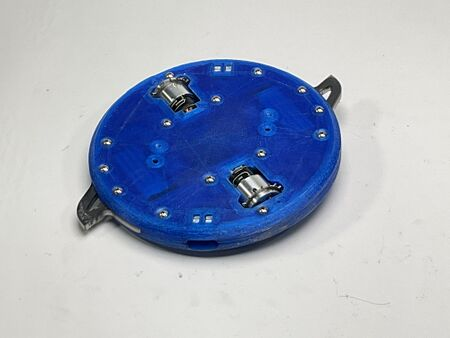
\includegraphics[scale=0.4]{deepmelt.jpg}
\caption{Deep Melt: Autonomous Melty Brain \cite{b2}}
\label{Deep Melt: Autonomous Melty Brain}
\end{figure}

Another autonomous battle bot is Orbitron, the first autonomous robot to appear on the show Battlebots, which works by essentially "orbiting" its opponent until it gets a "kill" command at which point it impacts its opponent to damage it \cite{b6}.  There is no mention of the planning algorithm used, however, when talking about the robot undesirably spinning along the robot's Z-axes when the weapon is turned on, "That's the whole reason we do it to spinners is that spin right there" \cite{b6} when referring to how the vertical spinners are mounted symmetrically on opposite sides of the robot, while spinning in opposite directions to eliminate the torque on the robot which causes the rotation.

\begin{figure}[htp]
\centering
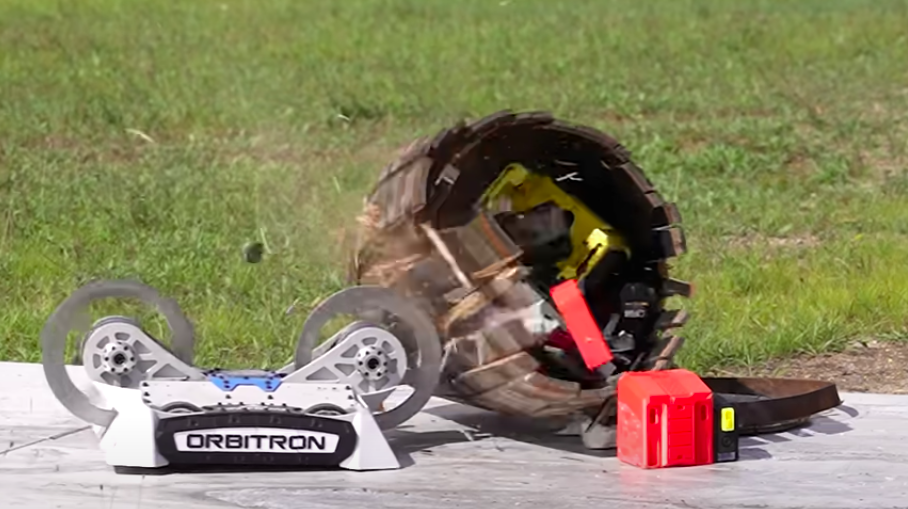
\includegraphics[scale=0.25]{orbitron.png}
\caption{Orbitron: Autonomous Vertical Spinner \cite{b6}}
\label{Orbitron: Autonomous Vertical Spinner}
\end{figure}

When looking at these autonomous battlebots there is one commonality, they are designed around autonomy.  Rather than being designed as a good robot first, and then making it autonomous, autonomous battlebots are designed to make control as easy as possible, however, it makes it impossible to generalize an autonomy system, since with these robots, the physical design of the robot is designed to make autonomy easier, rather than designing autonomy around existing robots.

\section{Creating the Kinodynamic Model}
In order to create a generalized kinodynamic planner for use in combat robotics, we first must create a generalized kinodynamic model of a combat robot.  We first must decide on its environment, since the vast majority of combat robots operate on the ground, with very few exceptions, we can model it in a 2 dimensional plane.  With this knowledge we can start with modeling the drive system of a robot, and since most robot drive systems can be modeled as a differential drive with the exceptions of the Melty Brains, which do not require a Kinodynamic model since they can be modeled as a point robot, and Swerve Drives, which are very rare with only 3 robots competing in the National Havoc Robotic League since 2018 as of May 2025\cite{b2}.  This means that we can cover the vast majority of combat robots by modeling all drive systems as a differential drive.  Of the differential drives we can create the force diagrams of the 2 types of differential drive, a 2 "wheel" drive (2WD), and a 4 "wheel" drive (4WD) as seen in the 2 models below where the "wheels" represent an locomotion method.  Additionally, by creating a force diagram of the weapon we can create a Kinodynamic model for a generalized combat robot.

\begin{figure}[htbp]
    \centering
    \begin{minipage}[b]{0.4\textwidth}
        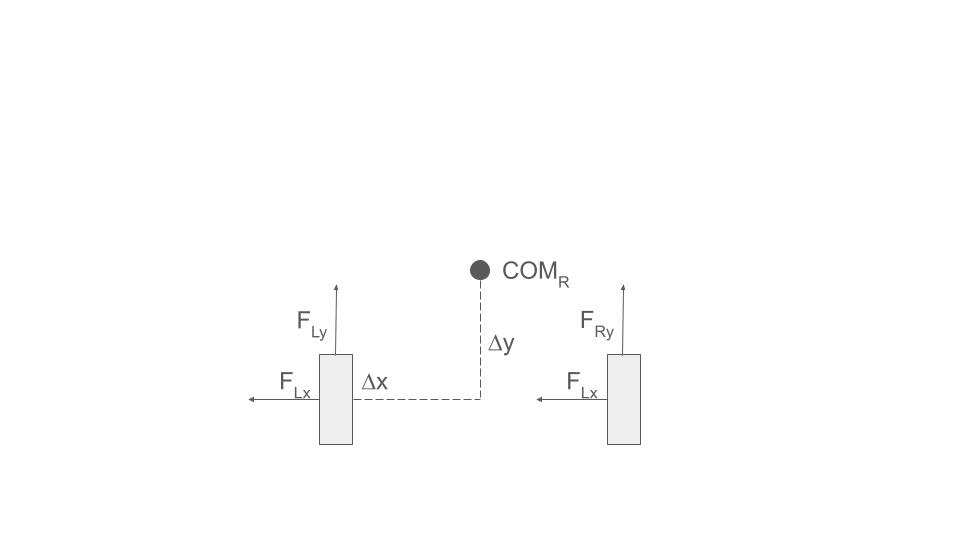
\includegraphics[width=\textwidth]{2WD.png}
        \caption{Force Diagram of a 2 Wheel Drive}
        \label{fig:rrt}
    \end{minipage}
    \hfill
    \begin{minipage}[b]{0.4\textwidth}
        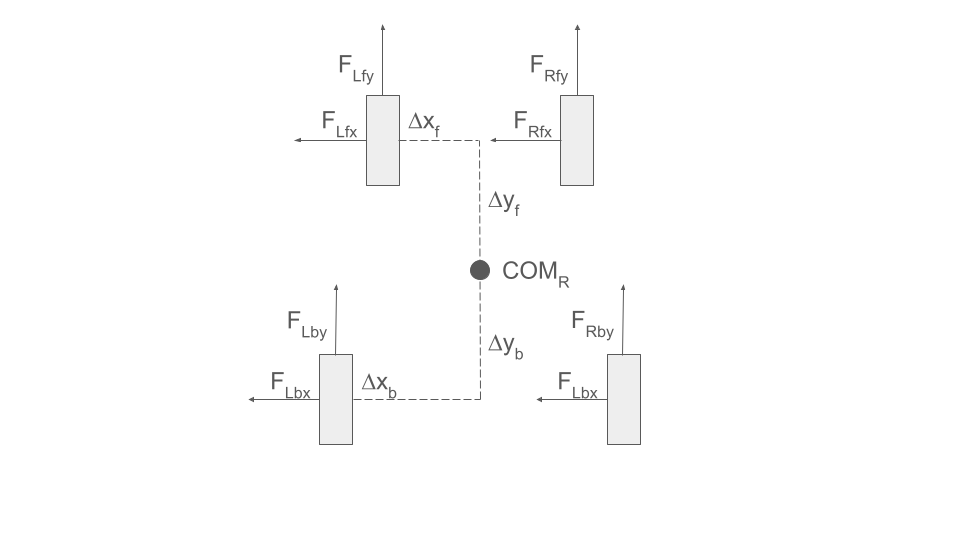
\includegraphics[width=\textwidth]{4WD.png}
        \caption{Force Diagram of a 4 Wheel Drive}
        \label{fig:kinorrt}
    \end{minipage}
    \hfill
    \begin{minipage}[b]{0.4\textwidth}
        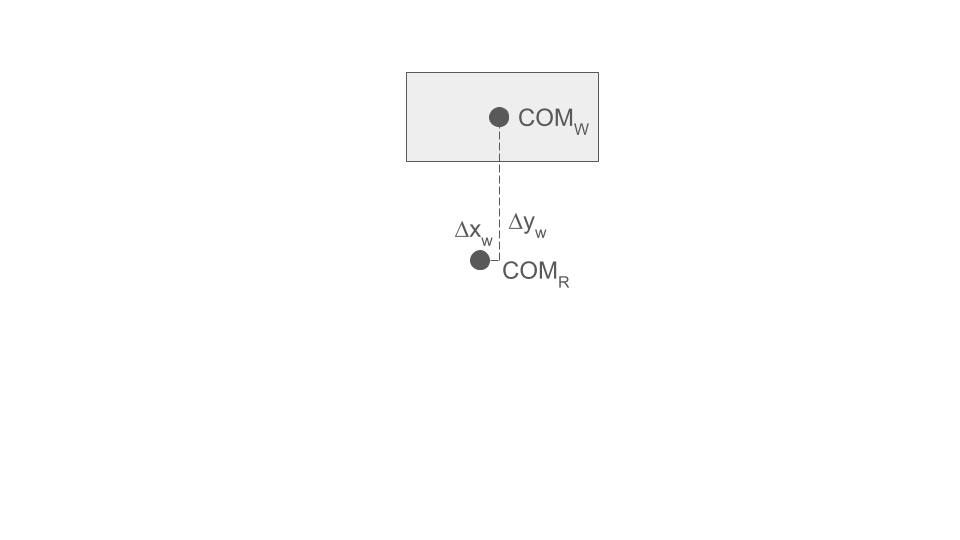
\includegraphics[width=\textwidth]{weapon.png}
        \caption{Force Diagram of a Battlebot's Weapon}
        \label{fig:kinorrt}
    \end{minipage}
*
\end{figure}

With the creation of the force diagrams, we can begin creating an example of a Kinodynamic model of a robot by deriving from known variables and our control space as shown below:
\begin{equation}
\mathcal{U} = \{PWM_L, PWM_R, PWM_W\}
\label{eq:control_space}
\end{equation}
\begin{equation}
PWM_L, PWM_R, PWM_W \in [-1,1]
\label{eq:control_space_dimensions}
\end{equation}

These 3 values represent the PWM or Pulse Width Modulation signal that go into the 3 relevant motors in the robot, the left drive motor, the right drive motor, and the weapon motor. By controlling the PWM signal the robot can control the torque each motor outputs.  Since the torque each motor outputs is known from the datasheets for each motor, and we know the inertial mass of the wheels and the weapon that the motors are turning we can also calculate the maximum angular acceleration for each motor in the robot using the generalized equation seen below:

\begin{equation}
\alpha_{max} = \frac{\tau}{I}
\label{eq:maximimum_angular_acceleration}
\end{equation}

Assuming that every wheel has the same known radius $r_{wheel}$ and same inertial mass $I_{wheel}$ where the tires have a coefficient of friction of $\mu_F$ with the calculated value of the maximum angular acceleration of the drive motors $\alpha_{maxDrive}$, in addition to the PWM values for the left and right drive motors $PWM_L$ and $PWM_R$  we can calculate the linear acceleration of the robot for both the 2WD and 4WD drive configurations using the equation below:


\begin{equation}
a_{linear}= \frac{\alpha_{maxDrive}\cdot r_{wheel} \cdot \mu_F \cdot (PWM_L + PWM_R)}{2}
\label{eq:linear_acceleration_calculation}
\end{equation}

After calculated the linear acceleration we must then calculate the force generated in the y and x axis of each wheel, the equations used with a generalized PWM value $PWM$ and the mass of the robot $m_{robot}$are shown below:

\begin{equation}
F_x = I_{wheel} \cdot  \alpha_{maxDrive} \cdot r_{wheel} \cdot PWM
\label{eq:X_direction_Wheel_Force}
\end{equation}

\begin{equation}
F_y = \frac{1}{2} \cdot m_{robot} \cdot I_{wheel} \cdot  \alpha_{maxDrive} \cdot r_{wheel} \cdot PWM
\label{eq:Y_direction_Wheel_Force}
\end{equation}

After finding the $F_x$ and $F_y$ values for every wheel in the robot, you then find the magnitude of the force tangent to a circle of a radius $\sqrt{\Delta x^2 + \Delta y^2}$ where $\Delta x$ and $\Delta y$ represent the distance from the center of mass of the robot in the x and y planes respectively.  Then you must calculate the tangent force that the wheel imparts on the circle, and lastly you must find the torque each wheel imparts on the robot.  Then by adding everything together you can get $\tau_{drive}$.  To calculate $\tau_{Weapon}$ you use the same method as for calculated the torque of a wheel except that $F_y=0$ in the case it is a vertical spinner, otherwise $\tau_{Weapon}=0$.  Lastly, to calculate the total torque on the robot you use the following equation, then using the torque and the total inertial mass of your robot $I_{robot}$ in the z axis you can find the angular acceleration of the robot $\alpha_{robot}$: 

\begin{equation}
\tau_{Robot} = \tau_{Drive} + \tau_{Weapon}
\label{eq:Total_Torque_Robot}
\end{equation}
\begin{equation}
\alpha_{Robot} = \frac{\tau_{robot}}{I_{robot}}
\label{eq:Angular_Acceleration_Robot}
\end{equation}

With the values $a_{linear}$ and $\alpha_{robot}$ it is possible to create the Kinodynamic model of the robot as seen below:

\begin{equation}
\mathbf{\ddot{q}} = 
\begin{bmatrix}
\ddot{x}_{robot} \\
\ddot{y}_{robot} \\
\ddot{\omega}_{robot} \\
\ddot{v}_{robot} \\
\ddot{\omega_{weapon}}
\end{bmatrix}
= 
\begin{bmatrix}
\dot{v}_{robot}cos(\theta) \\
\dot{v}_{robot}sin(\theta) \\
\ddot{\omega}_{robot} \\
\ddot{v}_{robot} \\
\ddot{\omega_{weapon}}
\end{bmatrix}
\end{equation}

\begin{equation}
\mathbf{\dot{q}} = 
\begin{bmatrix}
\dot{x}_{robot} \\
\dot{y}_{robot} \\
\dot{\omega}_{robot} \\
\dot{v}_{robot} \\
\dot{\omega_{weapon}}
\end{bmatrix}
= 
\begin{bmatrix}
{v}_{robot}cos(\theta) \\
{v}_{robot}sin(\theta) \\
\dot{\omega}_{robot} \\
\dot{v}_{robot} \\
\dot{\omega_{weapon}}
\end{bmatrix}
\end{equation}

\begin{equation}
\mathbf{q} = 
\begin{bmatrix}
{x}_{robot} \\
{y}_{robot} \\
{\omega}_{robot} \\
{v}_{robot} \\
{\omega_{weapon}}
\end{bmatrix}
\
\end{equation}

Of course, there is a maximum speed both linear and angular for all components determined by the hardware of the robot, with bounds in the x and y axis due to the arena the robot will be in.

\section{Representing the Arena}
In this paper we will be representing the arena used by Beetleweight or 3 lb robots in the National Havok Robotics League (NHRL).  According to the NHRL rulebook the arena is a 8'x8' wide square \cite{b2}, this sets the dimensionality of our experimental arena.  Additionally, we will be assuming that it is a real fight with a opponent with a constant velocity and a house bot that is also moving at a constant velocity.  The objective of the planner is to have our robot which starts at a randomized orientation, location, and velocity to simulate a portion of an actual fight.  The objective of our planner is to have our robot intercept the opponent with its weapon at maximum angular velocity while avoiding the housebot. In regards to the interception criteria it depends on the weapon type, the horizontal and vertical spinners must be at their maximum angular velocity on impact, while with the non-spinning weapons it is irrelevant, they just need to hit the opponent.

\begin{figure}[htp]
\centering
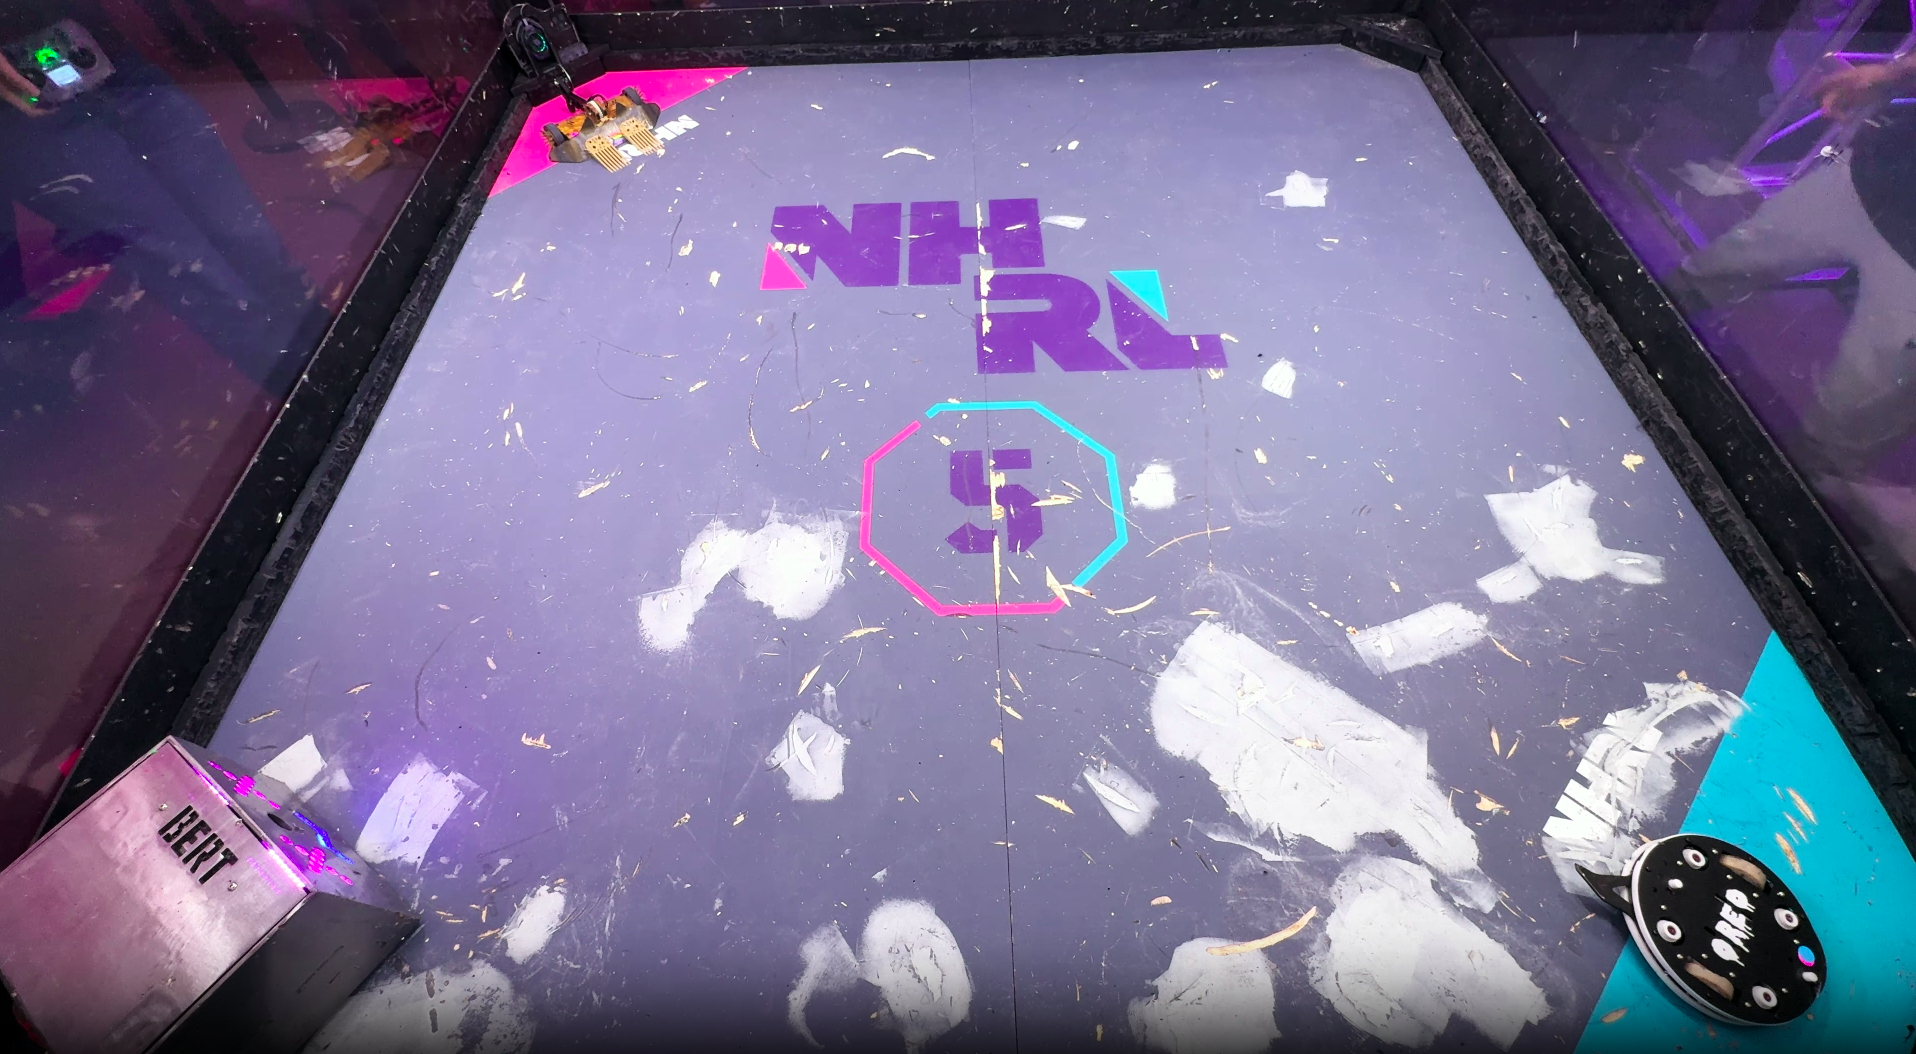
\includegraphics[scale=0.125]{arena.png}
\caption{Beetleweight Arena}
\label{Beetleweight Arena}
\end{figure}

\section{Evaluation}
To evaluate if the kinodynamic planning algorithm can truly function as a generalized kinodynamic planner for a wide variety of combat robots we will benchmark 6 separate configurations with 10 tests each on 5 separate planners, one for every potential combination of characterized drive system and weapon system which are all listed below:

\begin{enumerate}
\item{2WD Vertical Spinner}
\item{4WD Vertical Spinner}
\item{2WD Horizontal Spinner}
\item{4WD Horizontal Spinner}
\item{2WD Non-Spinning Weapon}
\item{4WD Non-Spinning Weapon}
\end{enumerate}

The path planning will take place in the Open Motion Planning Library (OMPL), the planners that will be benchmarked are Probabilistic Random Mapping (PRM), Rapidly-exploring Random Tree with Guidance (RG-RRT), Space-time RRT* (ST-RRT*), Rapidly-Exploring Random Tree (RRT), and Kinodynamic Planning by Interior-Exterior Cell Exploration (KPIECE1).  From this we will determine which one of these is the fastest, and if the average solve time is less than 2 seconds, we will consider it practical for usage with battle bots.


\newpage
\begin{thebibliography}{00}
\bibitem{b1} Berry, M. (2012, January). The history of robot combat: From humble beginnings to multinational sensation. Servo Magazine. https://www.servomagazine.com/magazine/article/the\_history\_of\_robot\_combat\_from\_humble\_beginnings.
\bibitem{b2} NHRL. (n.d.). https://wiki.nhrl.io/wiki/index.php?title=NHRL.
\bibitem{b3} Bruce Donald, Patrick Xavier, John Canny, and John Reif. 1993. Kinodynamic motion planning. J. ACM 40, 5 (Nov. 1993), 1048–1066. https://doi.org/10.1145/174147.174150.
\bibitem{b4} YouTube. (2025, February 17). What do you think they are dancing to?. YouTube. https://www.youtube.com/shorts/v5k6JwF7RNw.


\bibitem{b5} YouTube. (2022, December 8). Roomba x ChatGPT: Autonomous AI fighting robots, should we be worried?. YouTube. https://www.youtube.com/watch?v=Mr1YULNlAnE.


\bibitem{b6} YouTube. (2023, September 3). Building the First AUTONOMOUS BattleBot!? (VIDEO \#1/6)*. \text{https://www.youtube.com/watch?v=suv6DtRLnMw\&list=PLbncXbXlaNQemX6I22vQD6zWfIzIN9eOb}.





\end{thebibliography}

\vspace{12pt}



\end{document}
